\section{Image Reconstruction for Interferometers}\label{intro}
The angular resolution of a radio antenna is proportional to the wavelength divided by the dish diameter. To achieve high angular resolution the diameter should be as large as possible. But real world limitations like steering accuracy and price limit the diameter. Currently the largest single dish antenna has a diameter of about 500 meters\cite{chinaFAST}. 
  
Interferometers however, achieve high angular resolutions without the need for huge dish diameters. Several smaller antennas are spaced apart from each other. Together, they act as a single antenna. Interferometers have seen wide use in for the longer radio wavelengths with instruments like VLA, and LOFAR making numerous discoveries.

%The further the distance, the higher the maximum angular resolution the interferometer can achieve. several smaller antennas spaced apart from each other that act like a single large telescope.

Interferometers do not observe the sky directly. The observed image has to be reconstructed from the measurements. The reconstruction is an ill-posed inverse problem: There may be no unique solution and a small change in the measurements can lead to a big change in the reconstructed image. In Radio Astronomy, the CLEAN class of algorithms\cite{hogbom1974aperture}\cite{schwab1984relaxing}\cite{rich2008multi}\cite{rau2011multi} are used to reconstruct the image and is the de-factor standard. It is not guaranteed to reconstruct the true image in theory. In practice it has produced remarkable results with expert tuning. 

New instruments like MeerKAT make new type of observations. CLEAN is rigid and is not easily adapted to new observations.

The Theory of Compressed Sensing\cite{candes2006robust}\cite{donoho2006compressed} has seen success in solving ill-posed inverse problems. It is flexible in its application and can be used in de-noising\cite{many}, in-painting\cite{many} and super-resolution\cite{many}.

%Applying Compressed Sensing to wide Field of View imaging is an active field of research. In the last decade numerous approaches have been developed showing the potential of Compressed Sensing: Accurately modelling the effects of wide Field of View imaging, while reducing the tunable parameters and possibly super-resolved images\cite{garsden2015lofar}. Current research focuses on how the effects of wide Field of View can be accurately modelled while still being computationally efficient.

In this project, a proof of concept Compressed Sensing approach was developed and implemented in the Common Astronomy Software Application(CASA). 
%The approach is focused on small Field of View imaging and the reduction of expert intervention.

\subsection{Deconvolution: Ill-posed Inverse Problem}
Small field of view, the interferometer measures (almost) Fourier Components of the sky brightness. Inverse FFT works, it creates an image. Since but since it only measures a limited set of Fourier Components, the image is corrupted.

Try to find the true image from undersampled measurements. It is formulated as as a deconvolution problem: The corruption is modelled as a point spread function (PSF). The task is to deconvolve the dirty image, removing the corruption and restoring the original image.

\begin{equation}\label{intro:eq:deconvolve}
x \star  PSF + N = I_{dirty} 
\end{equation}

CASA produces a dirty image and a PSF.

In this project, the PSF models the instrumental effects of undersampling, antenna beam patterns. This problem 

%Each antenna pair measures a complex Visibility of the sky brightness. The distance between the antennas, the baseline, dictates the sample point in the Fourier Space (called UV-Space). Longer baselines sample higher frequency components, while shorter baselines sample lower frequency components. 

%For small Field of View imaging, the measured Visibilities equal two dimensional Fourier components. The observed image can be calculated by the two dimensional Inverse Fourier Transform. However the interferometer cannot sample the whole UV-Space. The image calculated by the Inverse Fourier Transform is 'dirty', it contains artefacts introduced by undersampling. 

\begin{figure}[h!]
	\centering
	\begin{subfigure}[b]{0.28\linewidth}
		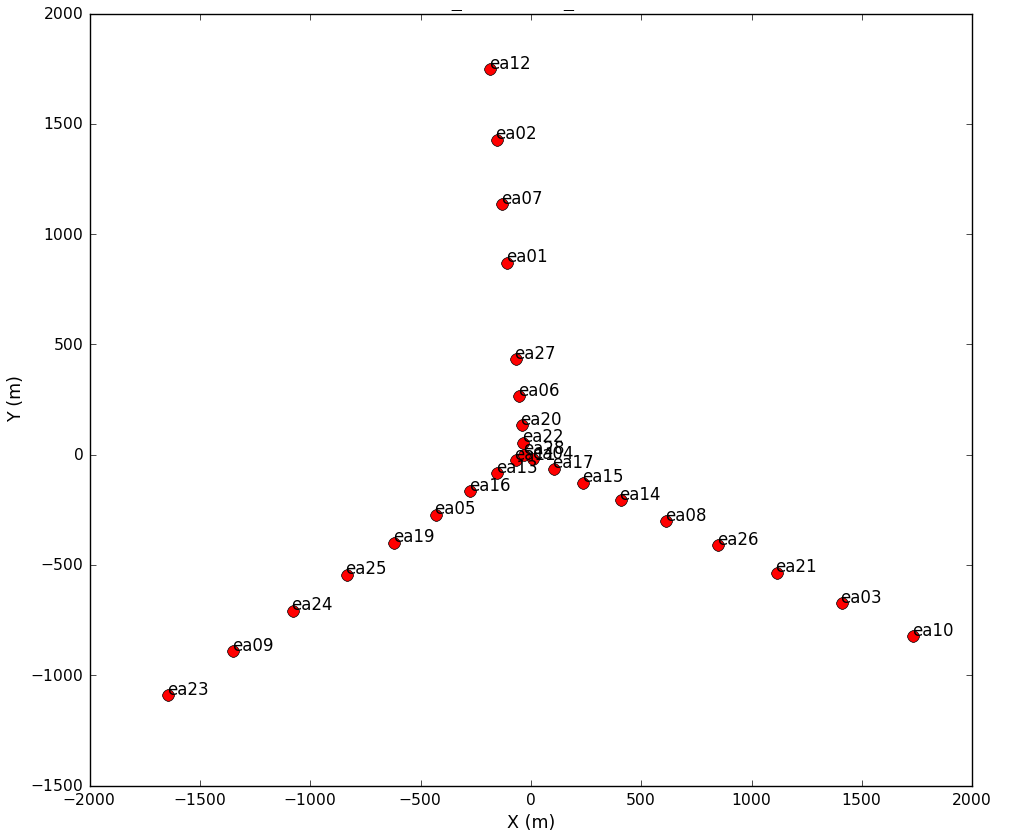
\includegraphics[width=\linewidth, trim={18px 19px 18px 18px}, clip]{./chapters/01.intro/img/antennas.png}
		\caption{Antenna Configuration}
	\end{subfigure}
	\begin{subfigure}[b]{0.28\linewidth}
		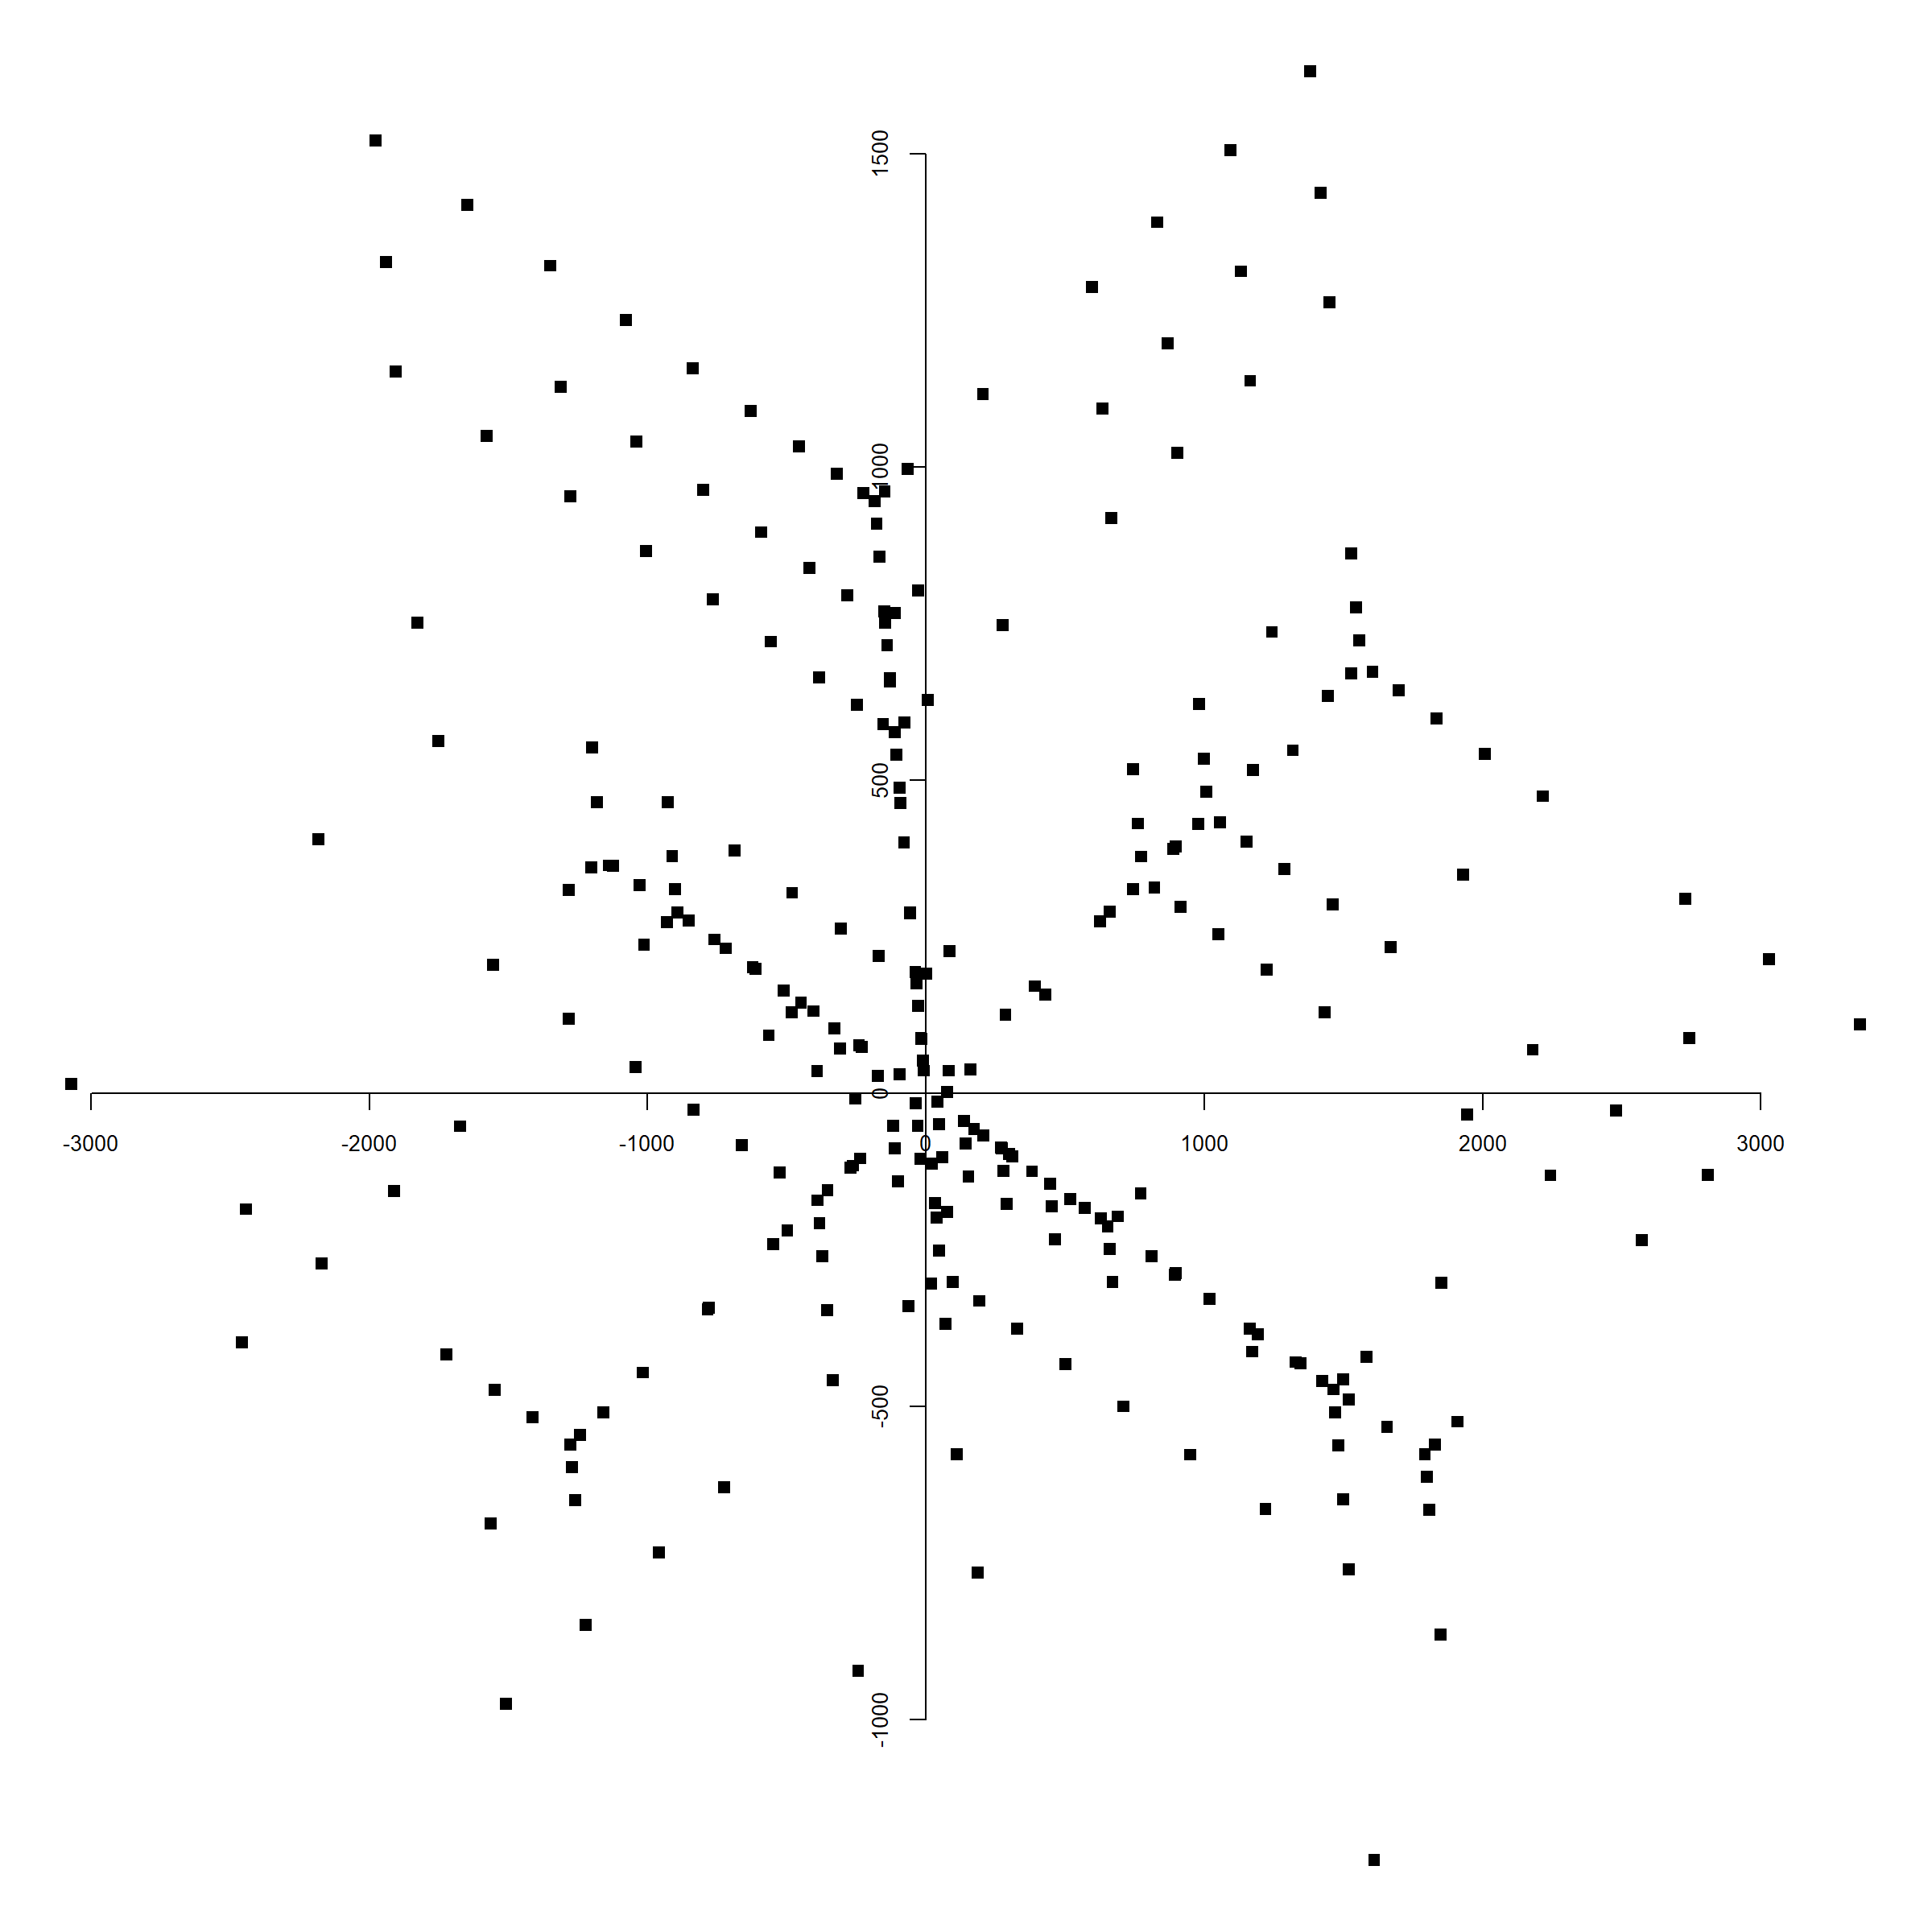
\includegraphics[width=\linewidth, trim={18px 19px 18px 18px}, clip]{./chapters/01.intro/img/uv.png}
		\caption{UV-Space}
	\end{subfigure}

	\begin{subfigure}[b]{0.28\linewidth}
		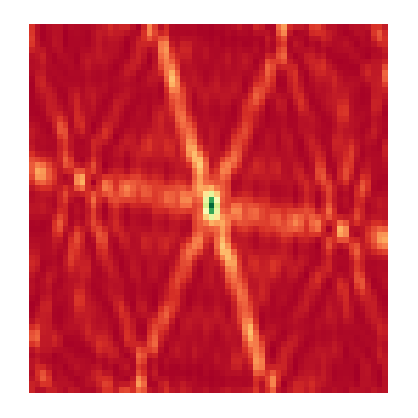
\includegraphics[width=\linewidth, trim={18px 19px 18px 18px}, clip]{./chapters/01.intro/img/psf.png}
		\caption{PSF}
	\end{subfigure}
	\begin{subfigure}[b]{0.28\linewidth}
		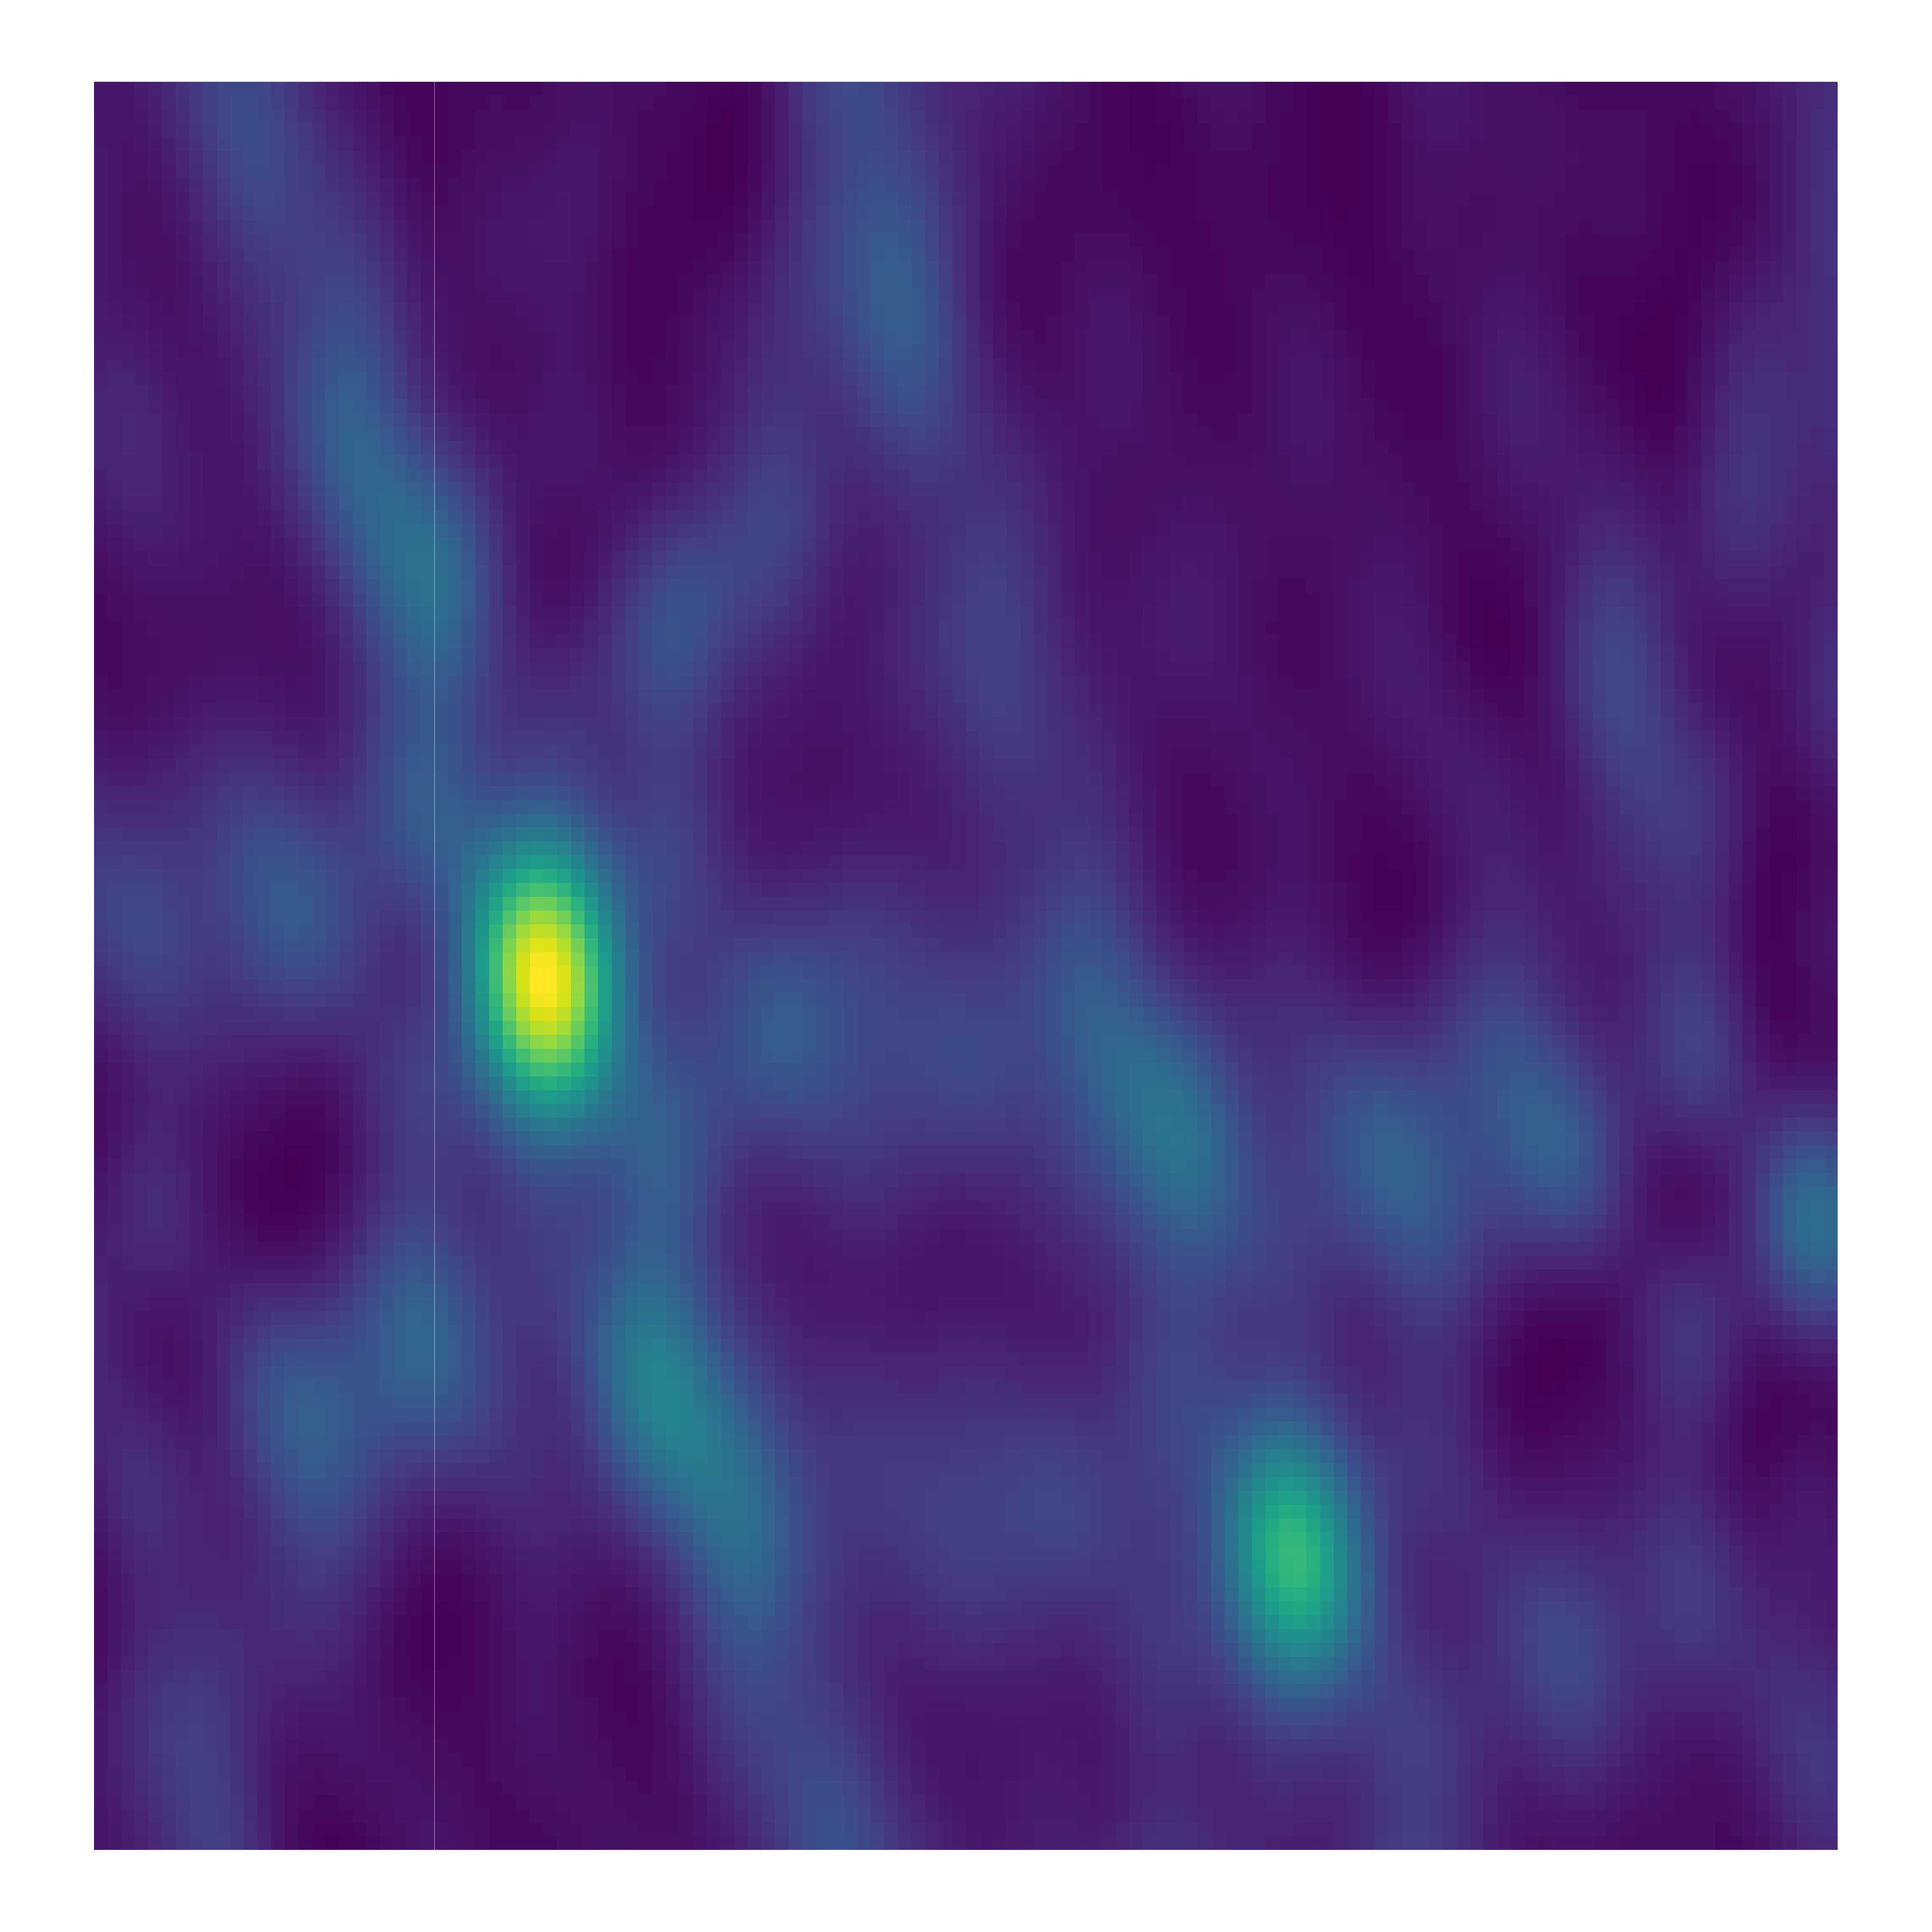
\includegraphics[width=\linewidth, trim={18px 19px 18px 18px}, clip]{./chapters/01.intro/img/dirty_image.png}
		\caption{dirty image}
	\end{subfigure}
	\begin{subfigure}[b]{0.28\linewidth}
		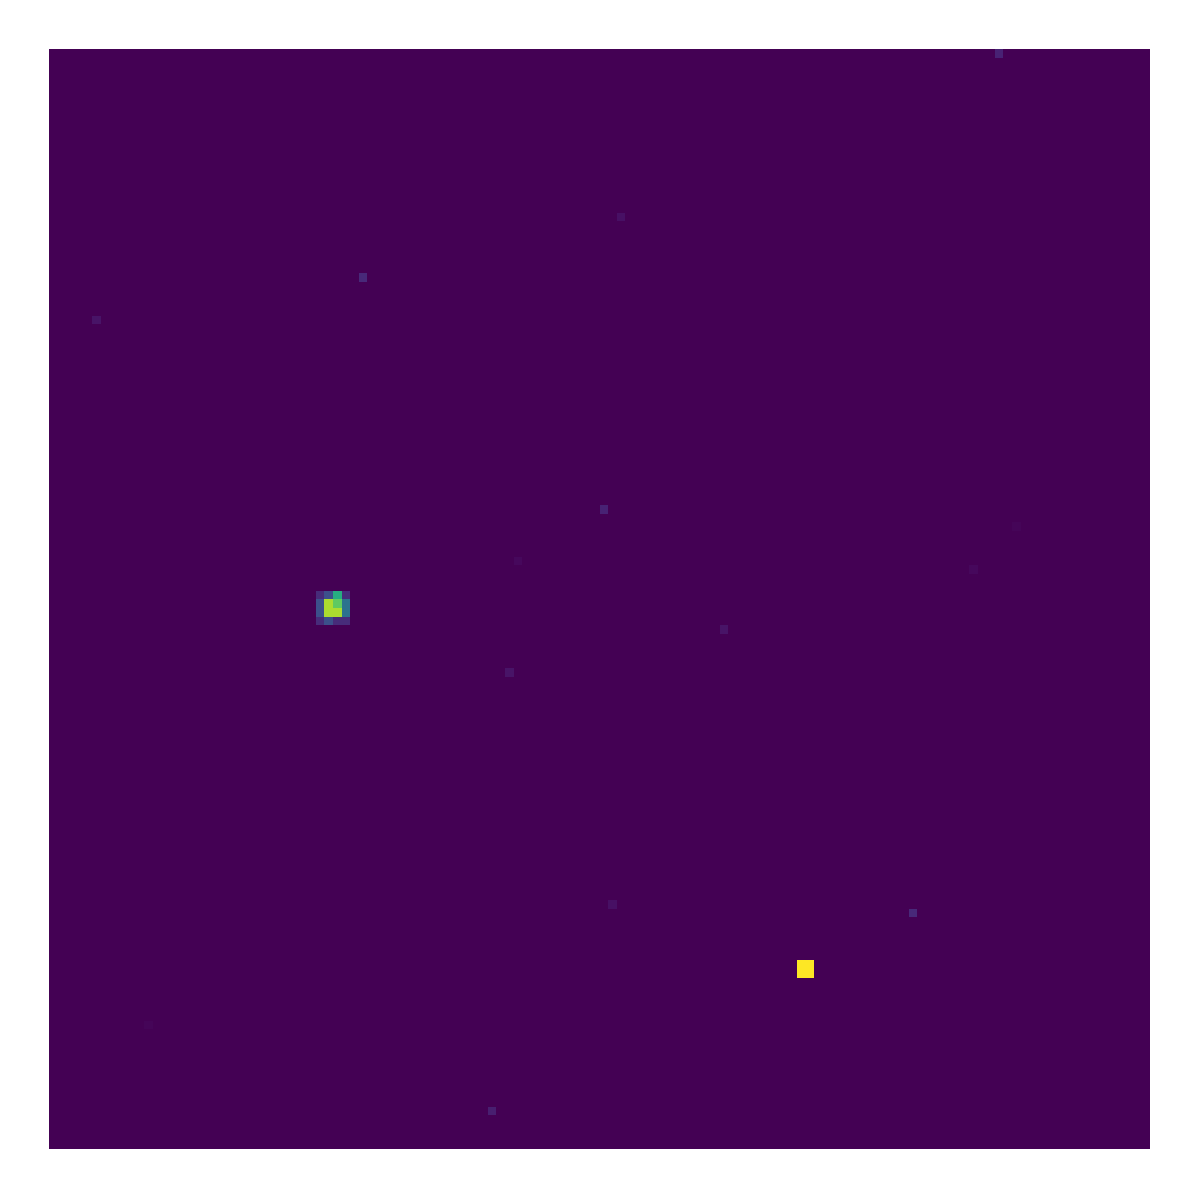
\includegraphics[width=\linewidth, trim={18px 19px 18px 18px}, clip]{./chapters/01.intro/img/true_image.png}
		\caption{true image}
	\end{subfigure}
	\caption{Deconvolution Problem VLA: Retrieve the true image when only PSF and dirty image are known}
	\label{intro:measurement_problem}
\end{figure}

%The Inverse Problem is now to remove the artefacts of the interferometer and retrieve the true image. The effects of the undersampling can be modeled by a Point Spread Function (PSF). The interferometer sees the true image of the sky, but due to undersampling it gets convolved with a PSF, resulting in the dirty image.  More formally, we try to find a solution $x$ for equation \eqref{intro:eq:deconvolve}, where only the PSF and $I_{dirty}$ are known. This problem is ill-posed: it may have multiple solutions, and a small change in the $I_{dirty}$ or the PSF may result in large changes in $x$. Furthermore, the whole problem gets corrupted by noise.

%The PSF is surprisingly easy to calculate. The Fourier Transformed PSF equals the sampling pattern in UV-Space. Remember that a convolution in image space is a multiplication in Fourier. The effects of under-sampling in image space are a convolution with the PSF. In the Fourier space it is masking all components other than the measured ones. From the Antenna Configuration we can infer the masking matrix $M$ in UV-Space. Calculating the Inverse Fourier Transform of $M$ results in the PSF.


\subsection{Approximation with CLEAN}
The idea of clean is that the image consists of point sources. A point source does 

In each iteration of CLEAN, it searches the highest peak of the dirty image and removing a fraction of the PSF at that point. It stops until the next highest peak is below a threshold, or if the maximum number of iterations was reached. The fraction of the PSF, threshold and number of iterations are all tunable by the user. State of the art implementations expose even more parameters. The reconstruction quality depends on the chosen parameters and require extensive user input.

CLEAN does not solve the deconvolution problem \eqref{intro:eq:deconvolve} directly. Instead, it greedily minimizes the objective \eqref{intro:eq:clean}. It is easy to see that if CLEAN minimizes the objective to zero, it has found a solution to the original deconvolution problem in a noiseless environment.

Note that the L0 norm\footnote{This is a common abuse of notation in Compressed Sensing literature: The "L0 norm" is not a norm.} acts as the indicator\footnote{For the L0 norm to work we need to define $0^0 = 0$} function.

\begin{equation}\label{intro:eq:clean}
\underset{x}{minimize} \: \left \| I_{dirty} - x \star PSF \right \|_2^2 + \: \lambda \left \| x \right \|_0
\end{equation}

Approximation of the problem.
%Since the original problem is ill-posed, the objective \eqref{intro:eq:clean} may have several zero points. In practice, CLEAN is stopped before it reaches zero. The addition of noise can add spurious peaks in the dirty image. By stopping early, CLEAN regularizes the objective. It assumes only a limited number of point sources exist in the image. The larger the magnitude of the peak, the more likely it is to be a real point source.

%In short, CLEAN does a greedy approximation of the deconvolution problem, and assumes the resulting image consists out of a few point sources. The question remains, how close the CLEAN approximation is to the true image? If the true image consists out of a few point sources, CLEAN produces a good approximation. Extended emissions however are harder for CLEAN to reproduce. The peak of extended sources is lower than that of point sources. It is harder for CLEAN to distinguish extended sources from noise.

T%he CLEAN regularization scheme is not ideal for extended sources. Ideally another way of regularization would be chosen for extended emissions, but the regularization is a fixed part of the CLEAN algorithm.


\subsection{The Compressed Sensing Framework for Image Reconstruction}

An image reconstruction algorithm in the Compressed Sensing Framework consists of three parts:

\begin{itemize}
	\item An objective with a data and regularization term.
	\item A prior function $p()$.
	\item An optimization algorithm.
\end{itemize}

The Prior $P$ transforms the image in a sparse domain. CLEAN assumes the $x$ contains a few point sources. In Compressed Sensing terminology, it assumes $x$ is sparse in image space. Since $x$ is already an image, the Prior $P$ in Compressed Sensing CLEAN is the identity matrix.

Clean in the cs framework
\begin{equation}\label{intro:eq:csclean}
\underset{x}{minimize} \: \left \| D_{dirty} - x \star PSF \right \|_2^2 \: + \: \lambda \: p(x) 
\end{equation}

The guarantees of Compressed Sensing Reconstruction: Incoherent from the measurement space and sparse space is sparse.

Incoherence is easy. Interferometers measure in the Fourier space(This is an approximation for small field of view imaging. The approximation breaks apart in wide field of view). The image space is maximally incoherent from the Fourier space. Intuitively, A change in a single pixel will change all fourier components. A change in a single fourier component, changes all pixels.

maximize the information gained for each element in the sparse space.

The sparse space is here to distinguish true image from unlikely candidates. It models our prior knowledge.

Then, one can reconstruct the true image from undersampled measurements. How many measurements are needed? that depends on how sparse it is. 

Taking again CLEAN as an example, if we know the image contains only one point source, we can locate it with only a few Visibilities. However if the image contains many point sources located closely together, we need more Visibilities.

The average case analysis is not trivial, 

%In the Compressed Sensing Framework, an approach is split into three separate parts. To demonstrate the flexibility of the Compressed Sensing Framework, we convert CLEAN into a Compressed Sensing approach.

% First we add a regularization term to \eqref{intro:eq:clean} and arrive at the new objective \eqref{intro:eq:csclean}. The objective contains the original CLEAN data term and a new regularization term. The data term forces the reconstruction to be close to the measurement, while the regularization term forces the reconstruction to be plausible. $\lambda$ models the expected noise in the problem. Note that the $\left \| Px \right \|_0$ acts as an indicator function. 

%The last step is choosing a similar optimization algorithm: In every iteration, CLEAN searches the highest peak in the dirty image. Matching Pursuit is a greedy optimization algorithm. In every iteration it searches the step which minimizes \eqref{intro:eq:csclean} the most. This Compressed Sensing approach is similar to CLEAN, but the new objective has a unique global minimum even with the presence of noise. The tunable parameters of CLEAN are replaced by a single parameter $\lambda$. 

%The strength of Compressed Sensing Framework is its flexibility: The CLEAN prior works well on point sources, but is not ideal for extended emissions. In this Framework, the prior $P$ can be replaced without changing the objective or the optimization algorithm. This has led to increased interest in Compressed Sensing for wide Field of View imaging.




